% fig_miplib_split: how BOBILib turns a single-level MILP into a bilevel instance.
% Checked on the instance files (all 389 MIPLIB-derived instances):
%  * miplib2010 / miplib2017 (Kleinert and Schmidt): the leader gets the first ceil(n/2)
%    variables in the order of the MPS file, the follower the rest.  X_0_100: every row
%    is a follower row.  X_50_50: the first ceil(m/2) rows are leader rows, the rest
%    follower rows; in 161 of the 163 _50_50 instances some leader row contains a
%    follower variable (a coupling row).  (The third variant, every row at the leader,
%    leaves the follower without rows; BOBILib has no such instance.)
%  * miplib3 (Fischetti et al.), X-k with k = 0.1, 0.5, 0.9: the follower gets the first
%    floor(k n) variables, the leader the rest; every row is a follower row.
%  * Objectives (every one of the 389): the leader keeps the MILP's objective c on all
%    variables; the follower's objective in the AUX file is -c on its own variables
%    (in 90 files written with six significant digits).
% Build: pdflatex fig_miplib_split.tex   (6.5 in x 2.0 in)
\documentclass[tikz,border=2pt]{standalone}
\pdfinfoomitdate=1 \pdftrailerid{} \pdfsuppressptexinfo=-1 % byte-identical rebuilds
\usepackage{mathptmx}
\usetikzlibrary{arrows.meta,calc}
\definecolor{leader}{HTML}{2A78D6}
\definecolor{follower}{HTML}{EB6834}
\definecolor{cert}{HTML}{1BAF7A}
\definecolor{ink}{HTML}{0B0B0B}
\definecolor{ink2}{HTML}{52514E}
\definecolor{muted}{HTML}{A9A8A2}
\definecolor{grid}{HTML}{E6E5E0}
\tikzset{
  every picture/.style={font=\fontsize{8}{9.6}\selectfont, color=ink, line cap=round, line join=round},
  small/.style={font=\fontsize{7}{8.4}\selectfont},
  ttl/.style={anchor=south west, inner sep=0pt, font=\fontsize{8}{9.6}\selectfont},
  lab/.style={font=\fontsize{7}{8.4}\selectfont, inner sep=0pt},
}
\def\MW{2.90}  % matrix width
\def\MH{1.95}  % matrix height
\def\SW{0.32}  % strip width
\def\my{1.48}  % bottom of the matrices
% \body{x0}: the matrix body at x0 (light grey), with its row strip to the left at x0-\SW-0.06
\newcommand{\body}[1]{\fill[grid] (#1,\my) rectangle ++(\MW,\MH);}
% \colstrip{x0}{from}{to}{colour}{label}{text colour}: part of the column strip above the matrix
\newcommand{\colstrip}[6]{%
  \fill[#4] (#1+#2*\MW,\my+\MH+0.06) rectangle (#1+#3*\MW,\my+\MH+0.06+\SW);
  \node[lab, text=#6] at (#1+#2*\MW/2+#3*\MW/2,\my+\MH+0.06+\SW/2) {#5};}
% \rowstrip{x0}{from}{to}{colour}{label}{text colour}: part of the row strip (from/to measured
% from the top of the matrix, as fractions)
\newcommand{\rowstrip}[6]{%
  \fill[#4] (#1-0.06-\SW,\my+\MH-#2*\MH) rectangle (#1-0.06,\my+\MH-#3*\MH);
  \node[lab, text=#6, rotate=90] at (#1-0.06-\SW/2,\my+\MH-#2*\MH/2-#3*\MH/2) {#5};}
% \hatch{x0}{y0}{x1}{y1}: dark grey 45-degree stripes (coupling block)
\newcommand{\hatch}[4]{%
  \begin{scope}
    \clip (#1,#2) rectangle (#3,#4);
    \foreach \t in {-3.0,-2.85,...,3.0}
      \draw[ink2, line width=0.45pt] (#1+\t,#2) -- ++(#4-#2,#4-#2);
  \end{scope}}
\begin{document}
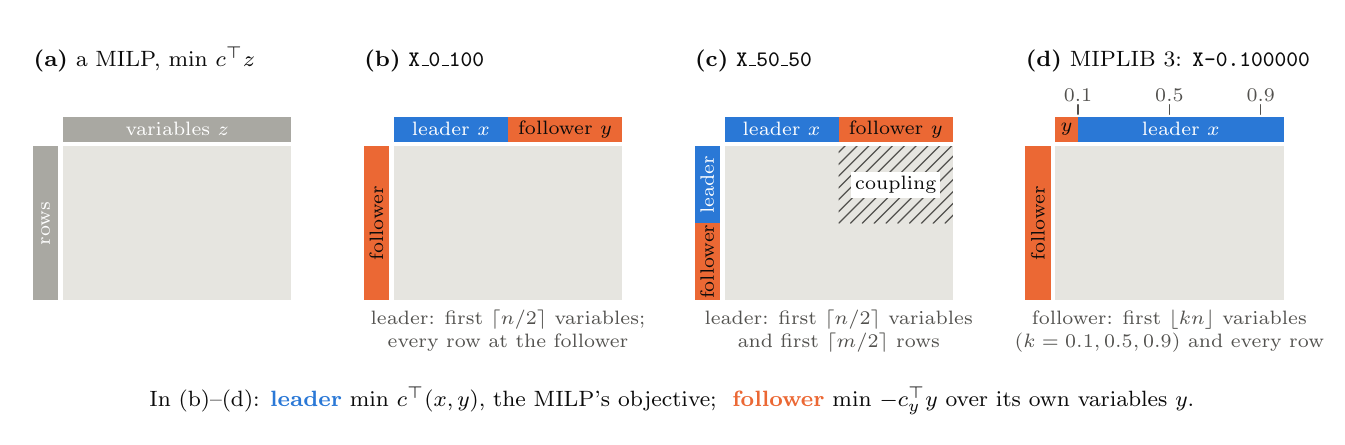
\begin{tikzpicture}
  % fixed page: 6.5 in x 2.0 in including the 2 pt border
  \useasboundingbox (0,0) rectangle (16.37,4.939);
  \def\Ttop{4.62}

  % ---------------- (a) the MILP ----------------
  \def\xa{0.45}
  \node[ttl] at (\xa-0.38,\Ttop-0.25) {\textbf{(a)} a MILP, $\min\, c^\top z$};
  \body{\xa}
  \colstrip{\xa}{0}{1}{muted}{variables $z$}{white}
  \rowstrip{\xa}{0}{1}{muted}{rows}{white}

  % ---------------- (b) X_0_100 ----------------
  \def\xb{4.65}
  \node[ttl] at (\xb-0.38,\Ttop-0.25) {\textbf{(b)} \texttt{X\_0\_100}};
  \body{\xb}
  \colstrip{\xb}{0}{0.5}{leader}{leader $x$}{white}
  \colstrip{\xb}{0.5}{1}{follower}{follower $y$}{ink}
  \rowstrip{\xb}{0}{1}{follower}{follower}{ink}
  \node[lab, anchor=north, text=ink2, align=center] at (\xb+0.5*\MW,\my-0.12)
    {leader: first $\lceil n/2\rceil$ variables;\\every row at the follower};

  % ---------------- (c) X_50_50 ----------------
  \def\xc{8.85}
  \node[ttl] at (\xc-0.38,\Ttop-0.25) {\textbf{(c)} \texttt{X\_50\_50}};
  \body{\xc}
  \hatch{\xc+0.5*\MW}{\my+0.5*\MH}{\xc+\MW}{\my+\MH}
  \node[lab, fill=white, inner sep=1.5pt] at (\xc+0.75*\MW,\my+0.75*\MH) {coupling};
  \colstrip{\xc}{0}{0.5}{leader}{leader $x$}{white}
  \colstrip{\xc}{0.5}{1}{follower}{follower $y$}{ink}
  \rowstrip{\xc}{0}{0.5}{leader}{leader}{white}
  \rowstrip{\xc}{0.5}{1}{follower}{follower}{ink}
  \node[lab, anchor=north, text=ink2, align=center] at (\xc+0.5*\MW,\my-0.12)
    {leader: first $\lceil n/2\rceil$ variables\\and first $\lceil m/2\rceil$ rows};

  % ---------------- (d) MIPLIB 3: X-k ----------------
  \def\xd{13.05}
  \node[ttl] at (\xd-0.38,\Ttop-0.25) {\textbf{(d)} MIPLIB 3: \texttt{X-0.100000}};
  \body{\xd}
  \colstrip{\xd}{0}{0.1}{follower}{$y$}{ink}
  \colstrip{\xd}{0.1}{1}{leader}{leader $x$}{white}
  \rowstrip{\xd}{0}{1}{follower}{follower}{ink}
  % where the split falls for k = 0.1, 0.5, 0.9
  \foreach \k in {0.1,0.5,0.9}
    \draw[ink2, line width=0.5pt] (\xd+\k*\MW,\my+\MH+0.06+\SW+0.03) -- ++(0,0.12)
      node[lab, anchor=south, text=ink2, inner sep=1pt] {\k};
  \node[lab, anchor=north, text=ink2, align=center] at (\xd+0.5*\MW,\my-0.12)
    {follower: first $\lfloor kn\rfloor$ variables\\($k=0.1, 0.5, 0.9$) and every row};

  % ---------------- objectives ----------------
  \node at (8.18,0.20)
    {In (b)--(d): \textcolor{leader}{\bfseries leader} $\min\, c^\top(x,y)$, the MILP's objective;
     \ \textcolor{follower}{\bfseries follower} $\min\, -c_y^\top y$ over its own variables $y$.};
\end{tikzpicture}
\end{document}
